\documentclass[a4paper]{report}
\usepackage[utf8]{inputenc}
\usepackage[portuguese]{babel}
\usepackage{hyperref}
\usepackage{a4wide}
\hypersetup{pdftitle={PCP - OpenMP e OpenMPI},
pdfauthor={João Teixeira, José Ferreira},
colorlinks=true,
urlcolor=blue,
linkcolor=black}
\usepackage{subcaption}
\usepackage{listings}
\usepackage{booktabs}
\usepackage{multirow}
\usepackage{appendix}
\usepackage{tikz}
\usepackage{authblk}
\usepackage{bashful}
\usepackage{verbatim}
\usepackage{amssymb}
\usepackage{multirow}
\usepackage{mwe}
\usepackage[parfill]{parskip}
\usetikzlibrary{positioning,automata,decorations.markings}
\AfterEndEnvironment{figure}{\noindent\ignorespaces}
\AfterEndEnvironment{table}{\noindent\ignorespaces}

\begin{document}

\title{Paradigmas de Computação Paralela\\Bucket Sort com OpenMP e OpenMPI}
\author{João Teixeira (A85504) \and José Filipe Ferreira (A83683)}
\date{\today}

\begin{center}
    \begin{minipage}{0.75\linewidth}
        \centering
        
\includegraphics[width=0.4\textwidth]{images/eng.jpeg}\par\vspace{1cm}
        \vspace{1.5cm}
        \href{https://www.uminho.pt/PT}
        {\color{black}{\scshape\LARGE Universidade do Minho}} \par
        \vspace{1cm}
        \href{https://www.di.uminho.pt/}
        {\color{black}{\scshape\Large Departamento de Informática}} \par
        \vspace{1.5cm}
        \maketitle
    \end{minipage}
\end{center}

\tableofcontents

\pagebreak

\chapter{Introdução}
O algoritmo escolhido para o projeto da unidade curricular de Computação
Paralela e Distribuída foi o \textit{Bucket Sort}.

Numa primeira fase do trabalho desenvolvemos uma versão sequencial do projeto e
procedemos ao \textit{benchmarking} do programa resultante. Em seguida
convertemos a implementação sequencial numa versão com utilização de memoria
partilhada fazendo uso de \textit{OpenMP} e comparamos o resultado com a versão
sequencial desenvolvida anteriormente. Posteriormente desenvolvemos uma nova
versao do \textit{bucket sort} fazendo uso de memoria distribuída com o
\textit{OpenMPI} comparando os resultados do benchmarking deste algoritmo
com os resultados obtidos na fase anterior.

Finalmente, nesta terceira fase do trabalho, iremos desenvolver uma nova versao
fazendo uso de uma arquitetura de memoria hibirda com o uso de \textit{OpenMP}
e \textit{OpenMPI}. Apresentando resultados dos benchmarkings realizados e
comparando-os com os resultados obtidos nas fases anteriores.

De notar que todos os benchmarks descritos foram efeutados em nós do tipo 641 do
cluster \textit{SeARCH}, e todos os executáveis foram compilados o
\textit{MPIcc} na versão 1.8.1 do \textit{OpenMPI}, utilizando a versão
7.2.0 do \textit{gcc}, e com as flags \textit{-fopenmp -O3 -std=c11} para garantir
a maior consistência entre os diferentes benchmarks. Na
ausência de indicação, os benchmarks foram efetuados com um input de 100000000
de elementos aleatórios, entre -1000 e 500000.

\chapter{Hibrido OpenMP OpenMPI} \label{chap:ompi}

\section{Descrição da Implementação}
Para esta implementação do algoritmo de Bucket Sort com utilização de um modelo
de memória hibirda, partimos do algoritmo desenvolvido para a versão feita sobre
\textit{MPI}, e utilizamos \textit{OpenMP} para paralelizar, dentro de cada
processo, a fase de construção dos baldes e a fase de ordenação destes.

\begin{figure}[h]
    \centering
    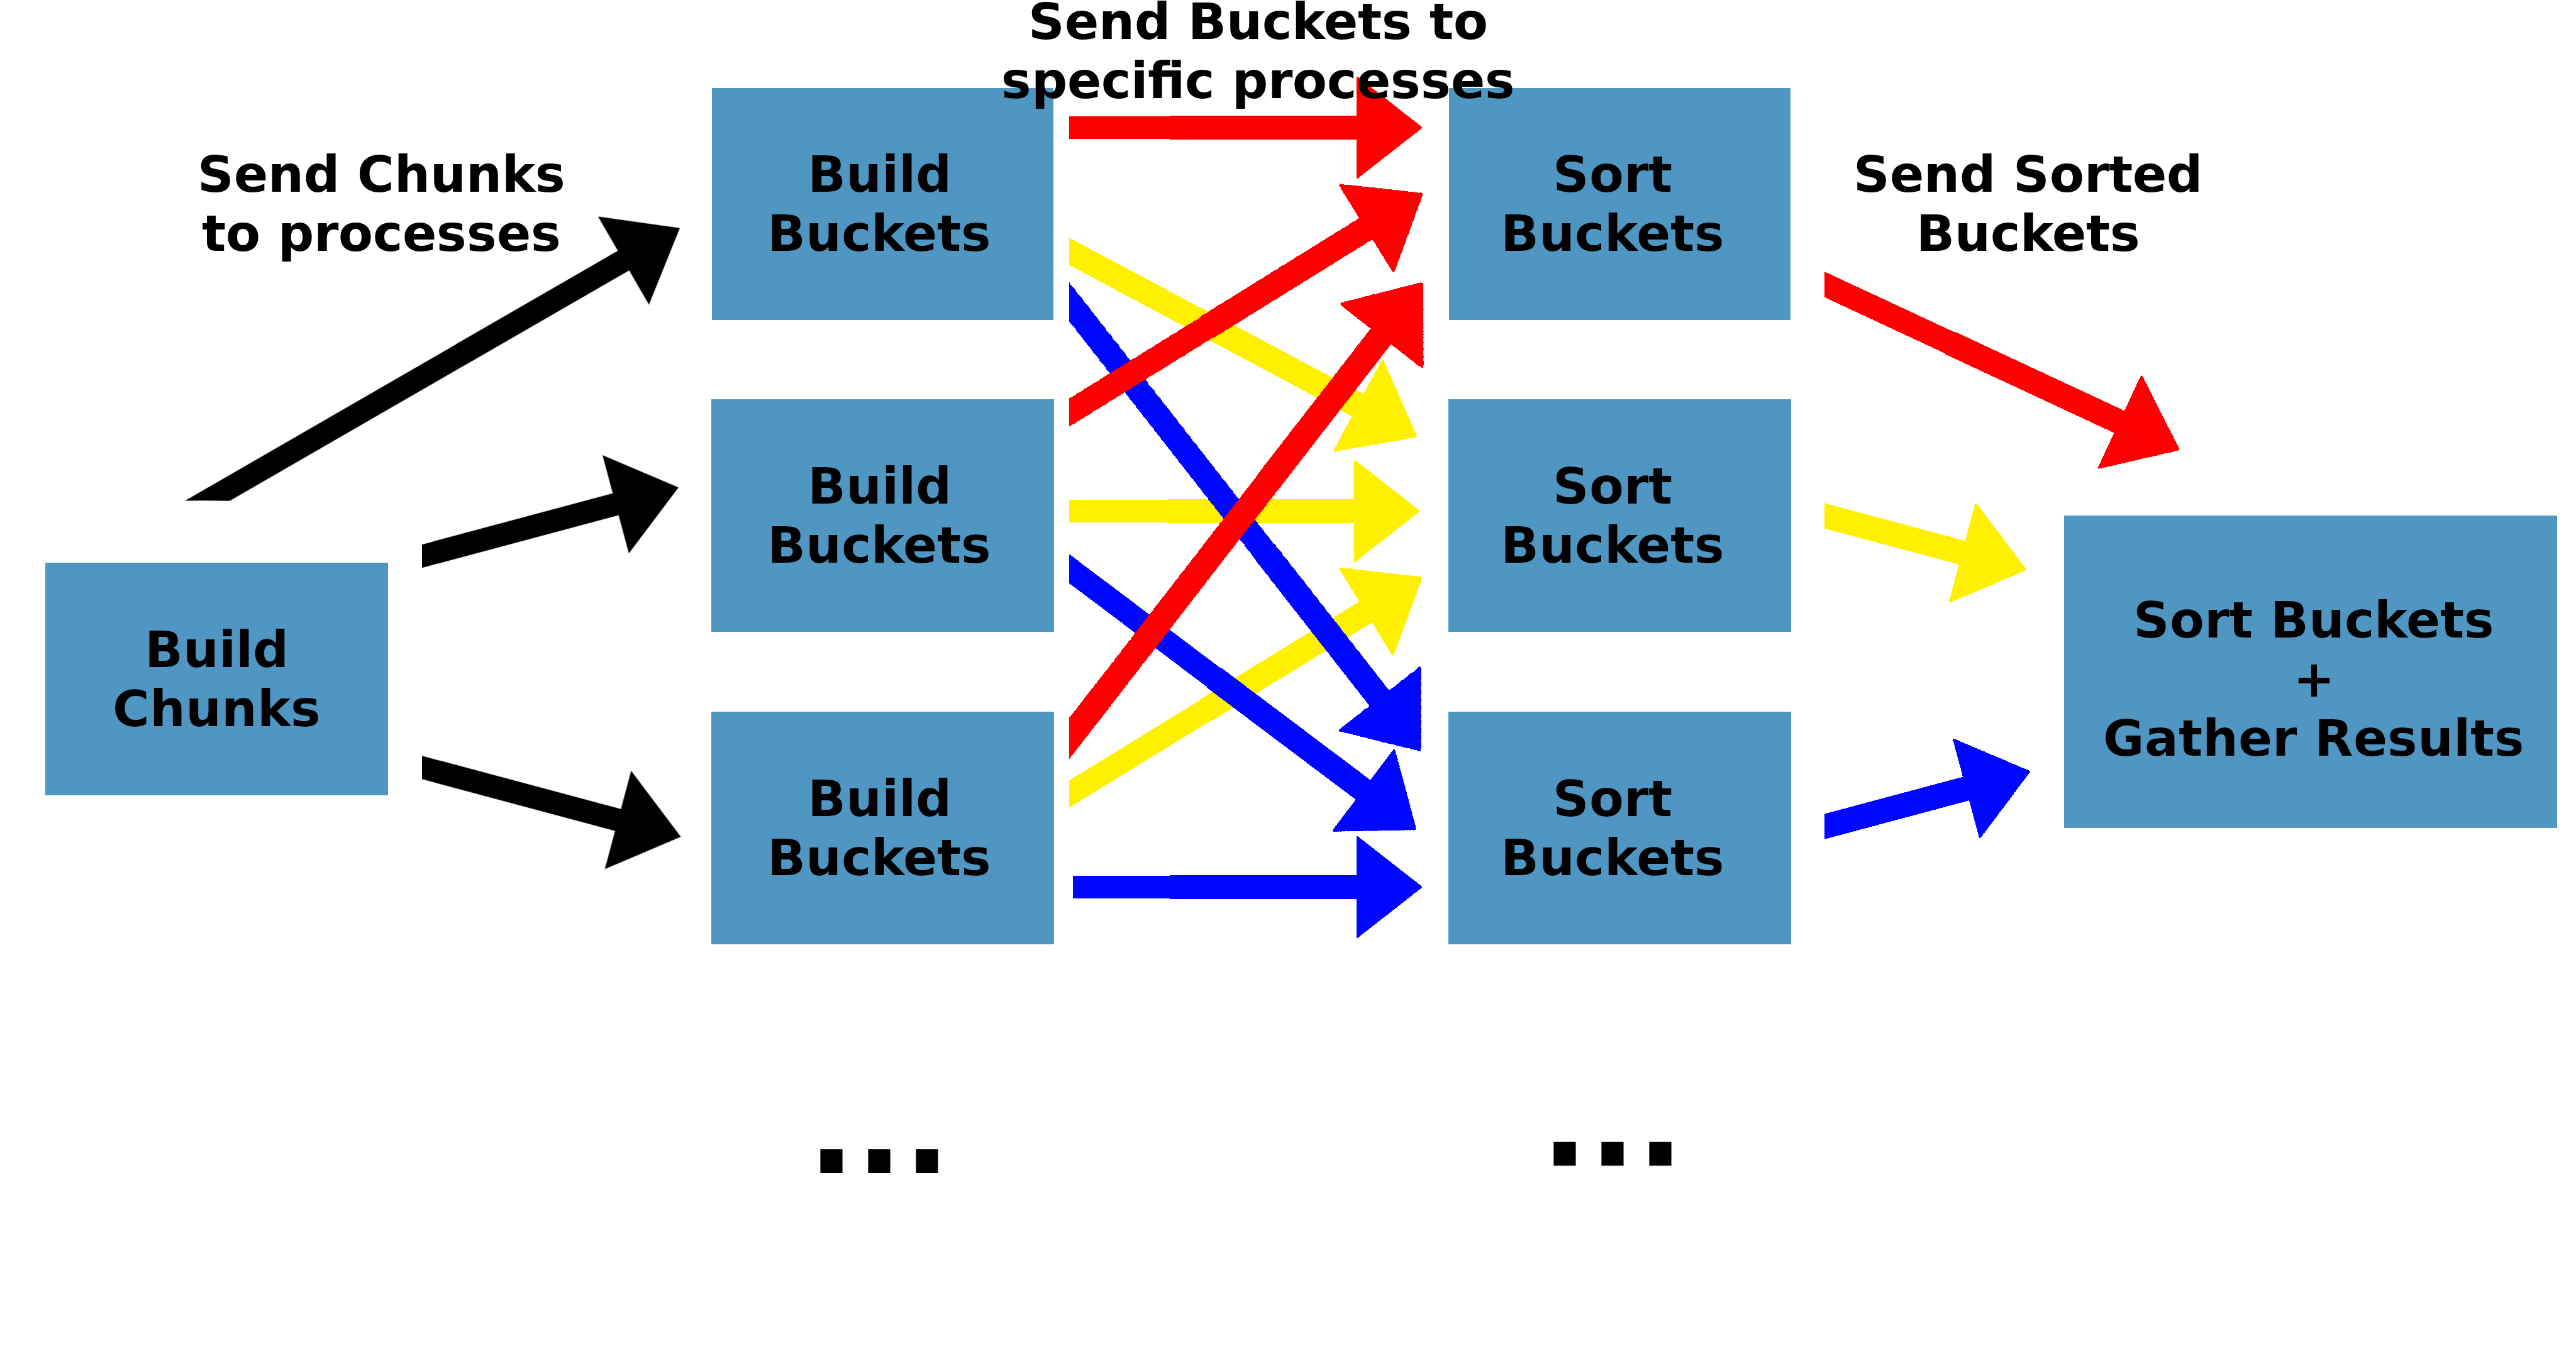
\includegraphics[width=0.6\textwidth]{images/esquemas/algoritmo_graph2.png}
    \caption{Arquitetura da Solução}
\end{figure}
\pagebreak

\section{Benchmarking e Análise dos resultados}

\subsection{Descrição dos Testes efetuados}
Com este modelo de memória hibrido, pretendemos encontrar um equilibrio entre o
custo de comunicação e de computação, tirando o máximo de partido da utilização
da memória partilhada dentro de cada processo MPI. Assim, efetuamos vários
testes, utilizando 32 cores de cada nodo, variando o número de processos MPI e
threads OMP de forma a encontrar o ponto ideal.

\subsection{Análise dos resultados obtidos}
\begin{table}[]
    \centering
    \begin{tabular}{|c|c|}
        \hline
        \multicolumn{2}{|c|}{Execution Times}                                                       \\ \hline
        \begin{tabular}[c]{@{}c@{}}4 processes by socket\\ (4 OMP threads)\end{tabular} & 8,850058  \\ \hline
        \begin{tabular}[c]{@{}c@{}}2 processes by socket\\ (8 OMP threads)\end{tabular} & 8,850058  \\ \hline
        \begin{tabular}[c]{@{}c@{}}1 process by socket\\ (16 OMP threads)\end{tabular}  & 14,353691 \\ \hline
        \begin{tabular}[c]{@{}c@{}}1 process by node\\ (32 OMP threads)\end{tabular}    & 23,873869 \\ \hline
        MPI only on 2 nodes                                                             & 20,496617 \\ \hline
        Sequential                                                                      & 16,209999 \\ \hline
    \end{tabular}
    \caption{Execution times by number of MPI processes}
    \label{tab:Times}
\end{table}
\begin{figure}[h]
    \centering
    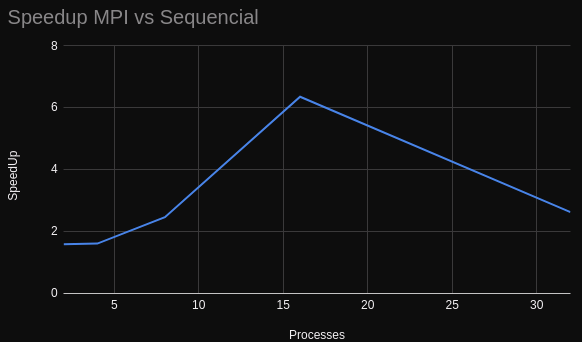
\includegraphics[width=0.6\textwidth]{images/speedupseq.jpeg}
    \caption{Speedup MPI vs Sequencial}
    \label{img:smpi}
\end{figure}

\end{document}
